\section{Recovering hidden marginals}
\label{sec:exclusiveViews}

\begin{figure}
  \centering
  \subfigure[Three-view mixture model] {
    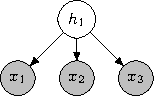
\includegraphics[width=0.45\columnwidth]{figures/three-view.pdf}
    \label{fig:three-view}
  }
  \subfigure[Exclusive views]{
    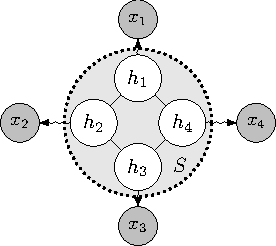
\includegraphics[width=0.45\columnwidth]{figures/exclusive-views.pdf}
    \label{fig:exclusive-views}
  }

  \caption{(a) The canonical three-view mixture model can be estimated consistently
  using tensor factorization \citep{anandkumar13tensor}.
  (b) An example of exclusive views for a bi-dependent subset $S$.
  }
\end{figure}


%In this section, we will develop a consistent parameter estimate for a class of directed graphical models.
%The conditional moments $\mOpp{v}{i} \eqdef \Pr(x_v \mid h_i)$
%recovered from {\TensorFactorize}, are not the underlying parameters.
  %Once we recover the conditional moments $\mOpp{v}{j} \eqdef \Pr(x_v
  %| h_j)$ for some $v, j$, we present a systematic approach to learn the
  %conditional probability tables for every clique for a class of directed
  %graphical models.
Having recovered conditional moments $\mOpp{v}{i} \eqdef \Pr(x_v \mid h_i)$,
we now seek to compute the marginal distribution of sets of hidden variables
$Z_S \eqdef \Pr(\bh_S)$.
%taking us one step closer to the actual model parameters.
%For clarity, we derive our algorithm in the infinite data limit,
%although the actual algorithm works with estimates.

%%%%%%%%%%%%%%%%%%%%%%%%%%%%%%%%%%%%%%%%%%%%%%%%%%%%%%%%%%%%
\subsection{Example: directed grid model}
\label{sec:directedExample}

To gain some intuition, consider the directed grid model from \figureref{approach}.
%The model has eight observed variables $x^a_1, x^b_1 \cdots, x^a_4, x^b_4$ and four
  %hidden variables $h_1, \ldots, h_4$.
The parameters of this model are the conditional probability tables
$\pi \eqdef \Pr(h_1) \in \Re^k, T \eqdef \Pr(h_2 | h_1) = \Pr(h_3 | h_1) \in \Re^{k \times k},
V \eqdef \Pr(h_4 | h_2, h_3) \in \Re^{k \times k \times k}$ and $O \eqdef \Pr(x^a_i | h_i)
=  \Pr(x^b_i | h_i) \in \Re^{d \times k}$. 

\paragraph{Estimating $O$}
Since the observed variables $x^a_1, x^b_1, x^a_2$ are
  conditionally independent given $h_1$, we can $\TensorFactorize$ from
  \sectionref{setup} to recover $O$.

\paragraph{Estimating $\pi$}
The moments of $x^a_1$, $\mO_1 \eqdef \Pr(x^a_1)$ are directly related to
  $\pi$ by a linear system: $\mO_1 = O \pi$. 
If $O$ has full column rank, we can recover $\pi$ by taking the pseudoinverse: $\pi = O\pinv  \mO_1$.

\paragraph{Estimating $T$}
Similarly, we can write down the moments of $x^a_1, x^a_2$, $\mO_{12}
  \eqdef \Pr(x^a_1, x^a_2)$, in terms of the hidden marginals $\mH_{12}
  \eqdef \Pr(h_1, h_2)$ and solve for $\mH_{12}$:
\begin{align*}
\mO_{12} = O \mH_{12} O^\top \quad\Rightarrow\quad
  \mH_{12} = O\pinv  \mO_{12} O\pinvt .
\end{align*}
$T$ can be recovered from the $\mH_{12}$ by renormalizing the columns.

\paragraph{Estimating $V$}
Finally, we can estimate $V$ by renormalizing the hidden marginals
$\mH_{234} \eqdef \Pr(h_2, h_3, h_4)$ from the third-order moments
$\mO_{234} \eqdef \Pr(x^a_2, x^a_3, x^a_4)$:
\begin{align*}
  \mO_{234} = \mH_{234}(O, O, O) \quad\Rightarrow\quad
  \mH_{234} = \mO_{234}(O\pinv , O\pinv , O\pinv ).
\end{align*}

%%%%%%%%%%%%%%%%%%%%%%%%%%%%%%%%%%%%%%%%%%%%%%%%%%%%%%%%%%%%
\subsection{Exclusive views}
\label{sec:general}

  %Section~\ref{sec:directedGeneral} will describe the algorithm in full generality.
%For ease of exposition we make the following simplifications to our presentation:
%(i) we describe our algorithm entirely in the context of directed
  %graphical models, though it generalizes to undirected models;
%(iii) we present the algorithm solely in terms of linear algebraic operations;
  %\sectionref{piecewise} provides a statistically
  %more efficient estimator using composite likelihood.

The intuitions of the directed grid generalize readily to general graphs.
The key property required for our algorithm to work is as follows:
\begin{definition}[Exclusive views]
  \label{def:exclusive-views}
Let $S \subseteq \bh$ be a subset of hidden variables.
We say $h_i \in S$ has an exclusive view $x_v$
  if the two conditions hold:
  (i) there exists some observed variable
  $x_{v}$ which is conditionally independent of the others $S \backslash \{ h_i \}$ given $h_i$,
  and (ii) the conditional moment matrix $\mOpp{v}{i} \eqdef
  \Pr(x_{v} \mid h_i)$ have full column rank $k$ and can be recovered.
We say that $S$ has the \emph{exclusive views property} if every $h_i \in S$ has an exclusive view.
%If every hidden clique has the exclusive views property, then we say that $\sG$ does as well.
\end{definition}

%%%%%%%%%%%%%%%%%%%%%%%%%%%%%%
\paragraph{Estimating hidden clique marginals}

We now show that if a subset of hidden variables $S$ has the exclusive views property,
then we can recover the marginal distribution $\Pr(\bh_S)$.
Consider any $S = \{i_1, \ldots, i_m\}$ with the exclusive views property. Let
  $x_{v_j}$ be an exclusive view for $h_{i_j}$ in $S$ and define $\sV
  = \{v_1, \ldots, v_m\}$. % be a set of exclusive views for the clique $S$.
By the exclusive views property,
the marginal over the observed variables $\Pr(\bx_\sV)$
factorizes according to the marginal over the hidden variables $\Pr(\bh_S)$
times the conditional moments:
\begin{align*}
  \mO_\sV 
  &\eqdef \Pr(\Sx{\sV}) \\
  &= \sum_{\vh_S} \Pr(\Sh{S}) 
                    \Pr(x_{v_1} | h_{i_1}) \cdots \Pr(x_{v_m} | h_{i_m}) \\
  &= Z_{S}(\mOpp{v_1}{i_1},\dots,\mOpp{v_m}{i_m}) \\
  &= Z_{S}(\mOppAll),
\end{align*}
where $\mOppAll = \mOpp{v_1}{i_1} \otimes \cdots \otimes \mOpp{v_m}{i_m}$ is the tensor product of
all the conditional moments.
Vectorizing, we have that
$Z_S \in \Re^{k^m}$,
$M_\sV \in \Re^{d^m}$,
and $\mOppAll \in \Re^{d^m \times k^m}$.
Since each $\mOpp{v}{i}$ has full column rank $k$,
the tensor product $\mOppAll$ has full column rank $k^m$.
Succinctly, $\mO_\sV$ (which can be estimated directly from data)
is a linear function of $Z_S$ (what we seek to recover).
We can solve for the hidden marginals $Z_S$ simply by projecting $\mO_\sV$ onto the column
space of $\mOppAll$:
\begin{align*}
  Z_{S} &= \mO_\sV(\mOpp{v_1}{i_1}\pinv,\cdots,\mOpp{v_m}{i_m}\pinv).
\end{align*}

\algorithmref{learnclique} summarizes the procedure, \LearnClique.
Given $Z_S$, the conditional probability tables for $S$ can easily be
obtained via renormalization.
\begin{theorem}[Hidden marginals from exclusive views]
If $S \subseteq \bx$ is a subset of hidden variables with the exclusive views property,
then \algorithmref{learnclique} recovers the marginals $Z_S = \Pr(\bh_S)$.
\end{theorem}

\begin{algorithm}
  \caption{\LearnClique~(pseudoinverse version)}
  \label{algo:learnclique}
  \begin{algorithmic}
    \REQUIRE Hidden subset $S = \{ h_{i_1}, \dots, h_{i_m} \}$ with exclusive views $\sV = \{ x_{v_1}, \dots, x_{v_m} \}$
    and $\{\mOpp{v_1}{i_i}\pinv\}$ % (\definitionref{exclusive-views})
    \ENSURE Marginal distribution $Z_S = \Pr(\bh_S)$.
      %\STATE Identify exclusive views $\Sx{\sV} = \{x_{v_1}, \dots, x_{v_m}\}$.
      \STATE Return $\mH_S \gets \mO_{\sV}( \mOpp{v_1}{i_i}\pinv, \dots, {\mOpp{v_m}{i_m}}\pinv )$.
  \end{algorithmic}
\end{algorithm}

%%%%%%%%%%%%%%%%%%%%%%%%%%%%%%
\paragraph{Structural properties}

We have shown how to estimate the parameters of any clique that possesses the exclusive
  views property (\definitionref{exclusive-views}).
  But in a general graph, which cliques have this property?
  To provide intuition, we will provide more interpretable sufficient conditions
  and examples.

% Define bidependent
First, define the notion of a bidependent set (in analogy with biconnected component),
in which conditionining on one variable does not break the set apart:
\begin{definition}[Bidependent set]
Given a graphical model $\sG$, we say that a subset of nodes $S$ is \emph{bidependent} if
conditioned on any $a \in S$, there is an active trail between any other two nodes $b,c \in S$.
\end{definition}
Note that all cliques are bidependent, but bidependent sets can have more conditional independences.
this will be important for pseudolikliehood in \sectionref{pseudolikelihood}.

% bidependent, bottleneck => exclusive views
Bidependent sets are significant because they guarantee exclusive views if they are bottlenecks:
%If a subset of hidden nodes $S$ is a bottleneck, it is clear that (ii)
%of the exclusive views property (\definitionref{exclusive-views}) via \TensorFactorize,
%but we will show that part (i) follows as well.
%Now we establish the link between bottlenecks and exclusive views:
\begin{lemma}[Bottlenecked implies exclusive views]
  \label{lem:bottleneck-views}  
  Let $S \subseteq \bh$ be a bidependent subset of hidden variables.
  If $S$ is a bottleneck, then $S$ has the exclusive views property.
\end{lemma}
\begin{proof}
Let $S$ be a bidependent subset and fix any $h_0 \in S$.
Since $h_0$ is a bottleneck, it has three conditionally independent views,
say $x_1, x_2, x_3$ without loss of generality. 
For condition (i), we will show that at least one of the views is conditionally independent
of $S \backslash \{ h_0 \}$ given $h_0$.
For the sake of contradiction, 
suppose that each observed variable $x_i$ is conditionally dependent on some
$h_i \in S \backslash \{h_0\}$ given $h_0$, for $i \in \{1, 2, 3\}$.
Then conditioned on $h_0$,
there is an active trail between $h_1$ and $h_2$ because $S$ is biconnected.
Thus, there is an active trail $x_1 - h_1 - h_2 - x_2$ conditioned on $h_0$.
Since the graphical model is faithful by assumption, we have $x_1 \not\perp x_2 \mid h_0$,
contradicting the fact that $x_1$ and $x_2$ are conditionally independent given $h_0$.
To show condition (ii), assume, without loss of generality, that $x_1$ is an exclusive view.
Then we can recover $\mOpp{1}{0} = \Pr(x_1 \mid h_0)$ via $\TensorFactorize$.
\end{proof}

%Note that bottlenecks provide three views, which is important for condition (ii) of
%\definitionref{exclusive-views}, only two is required for condition (i).
With this lemma in place, we present our full algorithm, $\LearnMarginals$,
in \algorithmref{directed}.

% DONE: move here because not central to story
\paragraph{Remarks.}
Note that even having two independent views for each $h_i \in S$ is sufficient for condition (i)
  of the exclusive views property, while three is needed for condition (ii).
The bottleneck property (\definitionref{bottleneck} can also be relaxed if some cliques
  share parameters.
For example, in the directed grid model, we can recover the conditional moments $O$ from
  $x^a_1, x^b_1$ and $x^a_2$ with $h_1$ as the bottleneck.
  Therefore, $h_2, h_3$ and $h_4$
  need not be bottlenecks, and we can omit the observations $x^b_2, x^b_3$ and $x^b_4$.

Our method also extends directly to case in which the observed variables
  are real-valued, while the hidden variables remain discrete. 
In this setting, the tensor factorization method of
  \citet{anandkumar13tensor} recovers the expected conditional means,
  $\mu_{vi} \eqdef \E(x_v | h_i) \in \Re^{d \times k}$ for each observed variable $x_v$ and
  hidden variable $h_i$.
\algorithmref{learnclique} and \algorithmref{directed} still apply and allow
  us to recover clique marginals $Z_\sC$.
%  \todo{make this a footnote if running out of space}
% PL: don't understand this comment
%In this case, we only require that the hidden variables in distinct
  %cliques share parameters.

\begin{figure}
  \centering
  \subfigure[Hidden Markov model] {
    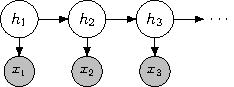
\includegraphics[width=0.45\columnwidth]{figures/hmm.pdf}
    \label{fig:examples-hmm}
  }
%  \subfigure[Directed grid model] {
%    \label{fig:examples-grid}
%    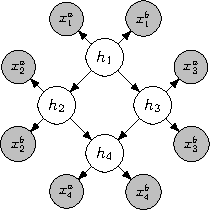
\includegraphics{figures/grid.pdf}
%  }
  \subfigure[Tree model] {
    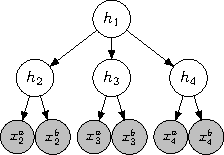
\includegraphics[width=0.45\columnwidth]{figures/tree.pdf}
    \label{fig:examples-tree}
  }
  \subfigure[Noisy-or model] {
    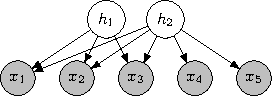
\includegraphics[height=5em]{figures/non-example.pdf}
    \label{fig:examples-noisy-or}
  }
  \caption{(a) and (b): graphs that satisfy the exclusive views property; (c) does not.}
  \label{fig:examples}
\end{figure}


\paragraph{Example: hidden Markov model.}

In the HMM (\figureref{examples-hmm}), the parameters
are $O \eqdef \Pr(x_i|h_i)$ and $T \eqdef \Pr(h_{i+1} | h_i)$
for all $i$.
While the first and last hidden variables $h_1, h_M$ in the
  sequence are not bottlenecks, they still have exclusive views ($x_1$ and
  $x_M$, respectively)
  due to parameter sharing.

\paragraph{Example: latent tree model.}

In the latent tree model (\figureref{examples-tree}), the parameters
are $\pi \eqdef \Pr(h_i)$, $T \eqdef \Pr(h_i | h_1)$ for $i \in \{2,3,4\}$,
and $O \eqdef \Pr(x^a_i | h_i) = \Pr(x^b_i | h_i)$ for $i \in \{2,3,4\}$.
Note that while $h_1$ is not directly connected to an observed variable,
  it is still a bottleneck, with views $x^a_2, x^a_3, x^a_4$.
We can recover $T$ from the clique $\{h_1, h_2\}$ by using views $x^a_2$
  (exclusive to $h_2$) and $x^a_3$ (exclusive to $h_1$).

\paragraph{Non-examples}
\label{sec:non-example}

There are certainly models which are identifiable but do not have exclusive views.
For example, \figureref{examples-noisy-or} shows
  a binary-valued noisy-or network which can be
  learned by the algorithm of \citet{halpern13noisyor},
  but does not satisfy the exclusive views property.

% %%%%%%%%%%%%%%%%%%%%%%%%%%%%%%
% \subsection{Sample complexity}
% \label{sec:sampleComplexity}
% PL: "combine" is too vague to be useful
%\LearnMarginals combines two consistent algorithms, \TensorFactorize and
%\LearnCliqueNs, and is thus consistent itself.

%In this section, we provide formal conditions under which $\LearnMarginals$
%will produce consistent estimates.
%We let
%$\mOpphat{v}{i}$,
%$\hat Z_\sC$,
%and $\hat M_\sV$,
%denote estimators for
%$\mOpp{v}{i}$,
%$Z_\sC$,
%and $M_\sV$,
%respectively.

% But $\mOpp{v}{i}$ is a product of tensors on the path from $h_i$ to
%   $x_v$, marginalizing out the rest of the graph.
% To make this property more interpretable, let us assume the following
%   property which we prove to be sufficient in
%   \appendixref{assumption-proof}:
% \begin{assumption} 
% \label{asm:full-rank-plus}
% The marginal distribution of every latent variable has full support:
%   $\forall{h_i \in H},~ \mPi{i} \succ 0$.
% For every clique $\sC \in \sG$ (including ones with observed variables),
%   and every conditional distribution $\Pr(h_c \given \Pa(h_c))$, where
%   $h_c \in \sC$, every {\em tensor unfolding} has full column rank, $k$.
% \end{assumption}
% In our directed grid example (\sectionref{directedExample}), for the
%   clique $\sC = \{ h_1, h_2 \}$ this condition implies $\pi = \Pr(h_1)
%   \succ 0$ and $T = \Pr(h_2 \mid h_1)$ has column rank $k$; for the clique
%   $\sC = \{ h_1, x_1 \}$, it implies $O = \Pr(x_1 \mid h_1)$ has column
%   rank $k$.

%\todo{did they prove this; if so just say "they show", not "we can show"}
%Using results from
%  \citet{anandkumar12moments,anandkumar13tensor} we can show that
%  learning $\mOpp{v_1}{i}$ for the bottleneck $h_i$ with views $x_{v_1},
%  x_{v_2}, x_{v_3}$ has the following sample complexity,
%  \todo{define hat O}
%  \todo{max subscript is misaligned}
%\begin{align*}
%  \|\mOpphat{v_1}{i} - \mOpp{v_1}{i}\|^2_F &= \frac{1}{\sqrt{n}} O\left( \frac{k {\pi\oft{i}}_{\max}^2}{\sigma_k(M_{v_1,v_2})^5} \right). 
%\end{align*}
%It is easy to see that $\LearnMarginals$ has a polynomial sample complexity because it composes two parts that individually have polynomial sample complexity.
%From \citet{anandkumar13tensor} given the non-degeneracy assumptions
%  \assumptionref{non-degeneracy}, we have that $\mOpphat{v}{i}$
%  converges to $\mOpp{v}{i}$ at a rate of $n^{-\frac12}$ with a constant
%  that depends polynomially on the $k$-th singular value of
%  $\mOpp{v}{i}$.
% PL: we don't have a crisp theorem (because there's multiple paths), so leave it vague.
%Recovering the marginals $Z_\sC$ from the conditional moments via $\LearnClique$ is a linear operation and thus also has polynomial sample complexity. 
%Note that $\sigma_{k}(\mOpp{v}{i})$ can become extremely
%small if $h_i$ and $x_v$ are connected via many intermediate hidden variables
%\footnote{To see this, consider a chain-structured graphical model: $h_1
%\to h_2 \cdots \to h_t \to x_v$. In this example, if
%$\sigma_k(\Pr(h_{i+1} \given h_{i})) \ge \sigma_k$ for each $i = 1,
%\cdots, t-1$, then $\sigma_k(\mOpp{v}{1})$ can be as bad as
%$\sigma_k^t \sigma_k(\mOpp{v}{t})$.}.
%\begin{theorem}[Sample complexity for $\mOpp{v}{i}$]
%  \label{thm:sample-complexity}
%  Without loss of generality, let $v=1, i=1$, and let $x_1, x_2, x_3$ be three views for
%  $h_1$. With probability at least $1 - \delta$,
%\begin{align*}
%  \|\mOpphat{1}{1} - \mOpp{1}{1}\|_F 
%    &\le  \\
%    &
%  \hspace{-0.3in}
%      O\left(
%      % PL: remove pi_max because that's upper bounded by 1.
%      \frac{k \log(1/\delta) } 
%      {\sqrt{n} \, \pi\oft{1}_{\min} (\sigma_{k}(\mOpp{1}{1}) \sigma_{k}(\mOpp{1}{2}))^{5/2}} \right),
%\end{align*}
%where $\pi\oft{1}_{\min}$ is the smallest element of $\pi\oft{1}$.

%If $\sigma_{\min}(\Pr(c \given \Pa(h_c))) \le \sigma$ for every clique
%  $\sC \in \sG$ and hidden variable $h_c \in \sC$,
%\begin{align*}
%  \|\mOpphat{1}{1} - \mOpp{1}{1}\|_F 
%    &\le 
%      O\left( 
%      \frac{k \log(1/\delta) {\pi\oft{1}}_{\max}/{\pi\oft{1}}_{\min}} 
%      {\sqrt{n} \sigma^{5t}} \right) \epsilon,
%\end{align*}
%where $t$ is the length of the shortest topological ordering from $h_1$
%to the unique parent of $x_1$, $h_t$.
%\end{theorem}
%In general, $\sigma_{k}(\mOpp{v}{i})$ will depend exponentially on the
  %path length between the hidden variable $h_i$ and $x_v$.
%This is expected because the influence from $h_i$ to $x_v$
  %gets diluted for every latent variable it must factor through.

%\theoremref{sample-complexity}, proved in \appendixref{assumption-proof}
%  says that the number of samples required to estimate the view
%  $\mOpp{v}{i}$ grows exponentially in the {\em distance} between $x_v$
%  and $h_i$. 

%\todo{Present sample complexity bounds for $Z_\sC$?}

% Easy case
% Next, we need to show that the hidden marginals $\hat Z_\sC$ converge to $Z_\sC$.
% First, $\hat M_\sV$ is just an empirical average of multinomials over the data points.
% Abusing notation slightly, we let $\hat M_\sV$ also denote its
% $d^{m}$-dimensional vectorized version.
% We also represent $\mH_\sC$ as
%   a vector in $\Re^{k^m}$, and represent $\mOppAll \eqdef
%   \mOpp{v_1}{i_1} \otimes \cdots \otimes
%   \mOpp{v_m}{i_m}$ as a matrix in $\Re^{d^m \times
%   k^m}$.
% By the central limit theorem, we have:
% $\sqrt{n} (\hat M_\sV - M_\sV) \convind \sN(0, \Sigma_\sV)$,
% where $\Sigma_\sV$ is the \emph{asymptotic variance} of $\hat M_\sV$: 
% % ARUN: I don't think so - \todo{doesn't this need to be multiplied by something?}
% \begin{align*}
% \Sigma_\sV \eqdef \dM_\sV - M_\sV M_\sV^\top, \quad \dM_\sV \eqdef \text{diag}(M_\sV).
% \end{align*}
% 
% Our next step will be to use the delta-method to convert the above
% result into the asymptotic variance for the pseudoinverse version of
% $\LearnClique$. 
% \begin{lemma}[Asymptotic variance of pseudoinverse estimator for $\tilde Z_\sC$]
%   \label{lem:mom-variance}  
%   Assume $\hat M_{\sV}$ has asymptotic variance $\Sigma_\sV$ defined above.
%   Then the asymptotic variance of $\hat{Z_\sC}$ is:
%   \begin{align*}
%     \Sigma^{\mom} &= \mOppAlli \Sigma_\sV \mOppAllit.
%   \end{align*}
%   %where ${\mOppAll}\pinv \eqdef {\mOpp{v_1}{i_1}}\pinv \otimes
%   %\cdots \otimes {\mOpp{v_m}{i_m}}\pinv$, a $d^m \times k^m$ matrix.
% \end{lemma}
% \begin{proof}
% For clique $\sC$, recall we have
%   $Z_{\sC} = \mO_\sV(\mOppi{v_1}{i_1},\cdots,\mOppi{v_m}{i_m})$.
% %Choosing to represent $Z_\sC$ and $M_\sV$ as vectors and
% %$\mOppi{v_1}{i_1} \otimes \cdots \otimes \mOppi{v_m}{i_m}$ as the
% %matrix,
% We can rewrite this representation more compactly as: $Z_{\sC} = {\mOppAll}\pinv \mO_\sV$.
% By the delta-method \cite{vaart98asymptotic},
% % DONE: need to shorten
% %we have that the asymptotic variance of $M_\sV$ is:
% %\begin{align*}
% %  \sqrt{n}(\hat M_\sV - M_\sV) \convind \sN(0, \Sigma_\sV),
% %\end{align*}
% %where $\Sigma_\sV$ is the variance of the observations. 
% we immediately get:
% $\sqrt{n}(\hat Z_\sC - Z_\sC) \convind \sN(0, \mOppAlli \Sigma_\sV \mOppAllit)$.
% \end{proof}

% DONE: too brazen to say
%Note that extending these results to finite sample bounds can be done
  %via a straightforward application of perturbation bounds.
